\chapter{Methodology}
\label{sec:methodology}

% This chapter enumerates and discusses the specific steps and activities that will be performed by the proponent to accomplish the objectives of the research. The discussion covers the activities from pre-proposal to Final Thesis Writing. 

% Ethical issues surrounding the research and the steps to be taken by the research team to adhere to ethical guidelines and principles should be included when discussing each of the activities.

% Research activities include inquiry, survey, research, brainstorming, canvassing, consultation, review, interview, observe, experiment, design, test, document, and other similar tasks. The following sections present an example set of activities and methods for conducting computing research. \textbf{\textcolor{red}{However, note that your group's actual research activities and methods will be different depending on your intended research contributions. You should consult closely with your thesis adviser for proper guidance. The following sections need not appear in your actual thesis proposal.}}

% \section{Data Collection}

% This section, also called "Data Gathering", focus on activities that will enable the researchers to understand their users and their context better, or to analyze the operating environment where the proposed software may be deployed. The types of activities would include interviews, observations, surveys, focus group discussions, and review of secondary data (reports, videos, manuals) to enable the researchers to identify user requirements; learn the existing processes, strategies, rules and guidelines; and/or build the datasets and knowledge resources needed in the study.

% Ethical issues surrounding the collection of data from human participants, and from internet or 3rd party sources should be indicated. The steps to be taken by the proponents to ensure that ethical guidelines are followed should also be explained.

% \section{Software Design and Implementation}

% This section covers the design of data structures, knowledge bases, user interface, and algorithms. It includes implementation and related activities - tool selection, unit testing, integration testing, and function testing - that were covered in the course "Software Engineering".

% Your Adviser may ask you to separate the Design and the Implementation sections as needed. 

% You may also indicate a specific software development lifecycle model that you plan to adopt in developing your software, such as the Agile methodology.

% For machine learning types of research, this section may be replaced with "Model Training".

% \section{Validation}

% This section contains the different types of validation activities that you will conduct to evaluate the performance of your model or algorithm or software. It may include user perception studies, end user acceptance testing, usability test, and model validation.

% Ethical issues surrounding the collection of data from human participants should be indicated. The steps to be taken by the proponents to ensure that ethical guidelines are followed should also be explained.

% This section should include a discussion of the following if working with human participants:
% \begin{itemize}
%     \item Participant Selection. Who are your target participants? How will they be selected? What data will be collected?
%     \item Orientation. How will ethics be observed? What documents, e.g., validation protocol, will be shared with participants to orient them regarding the research and the validation procedure? Will there be an Informed Consent and Informed Assent? Are they found in the Appendix? Will there be any pre-tests or interviews to be administered prior to the actual experiment?
%     \item Experiment Proper (aka Procedure). How long is the experiment or how long should the user use your software? Is it one-on-one, or one-to-many? What will you do while the experiment is ongoing - observe the participants using a checklist, guide the participants, record the interaction/usage?
%     \item Debriefing. After the experiment, will you administer any post-tests or debriefing to solicit feedback from your participants? What are these?
% \end{itemize}

% \subsection{Calendar of Activities}

% For the proposal, a Gantt chart showing the schedule of the activities should be added. You can create a table like below, or create a figure. For example:

% Table \ref{tab:timetableactivities} shows a Gantt chart of the activities.  Each bullet represents approximately one week worth of activity.

% \begin{table}[]
%     \centering
%     \begin{tabular}{l|c|c|c|c|c|c|c|c|c}
%          \toprule
%          & \multicolumn{6}{c|}{2021} & \multicolumn{3}{c}{2022} \\
%          \textbf{Activity} & \textbf{Apr} & \textbf{May} & \textbf{Jun} & \textbf{Jul} & \textbf{Aug} & \textbf{Sep} & \textbf{Jan} & \textbf{Feb} & \textbf{Mar} \\
%          \midrule
%          Data Collection & **** & **** & & & & & & & \\
%          \midrule
%          Software Design & & **** & **** & **** & **** & **** & & & \\
%          \midrule
%          Validation & & & & & & **** & **** & **** & \\
%          \bottomrule
%     \end{tabular}
%     \caption{Gantt Chart of Activities}
%     \label{tab:timetableactivities}
% \end{table}

\begin{figure}[h]
    \centering
    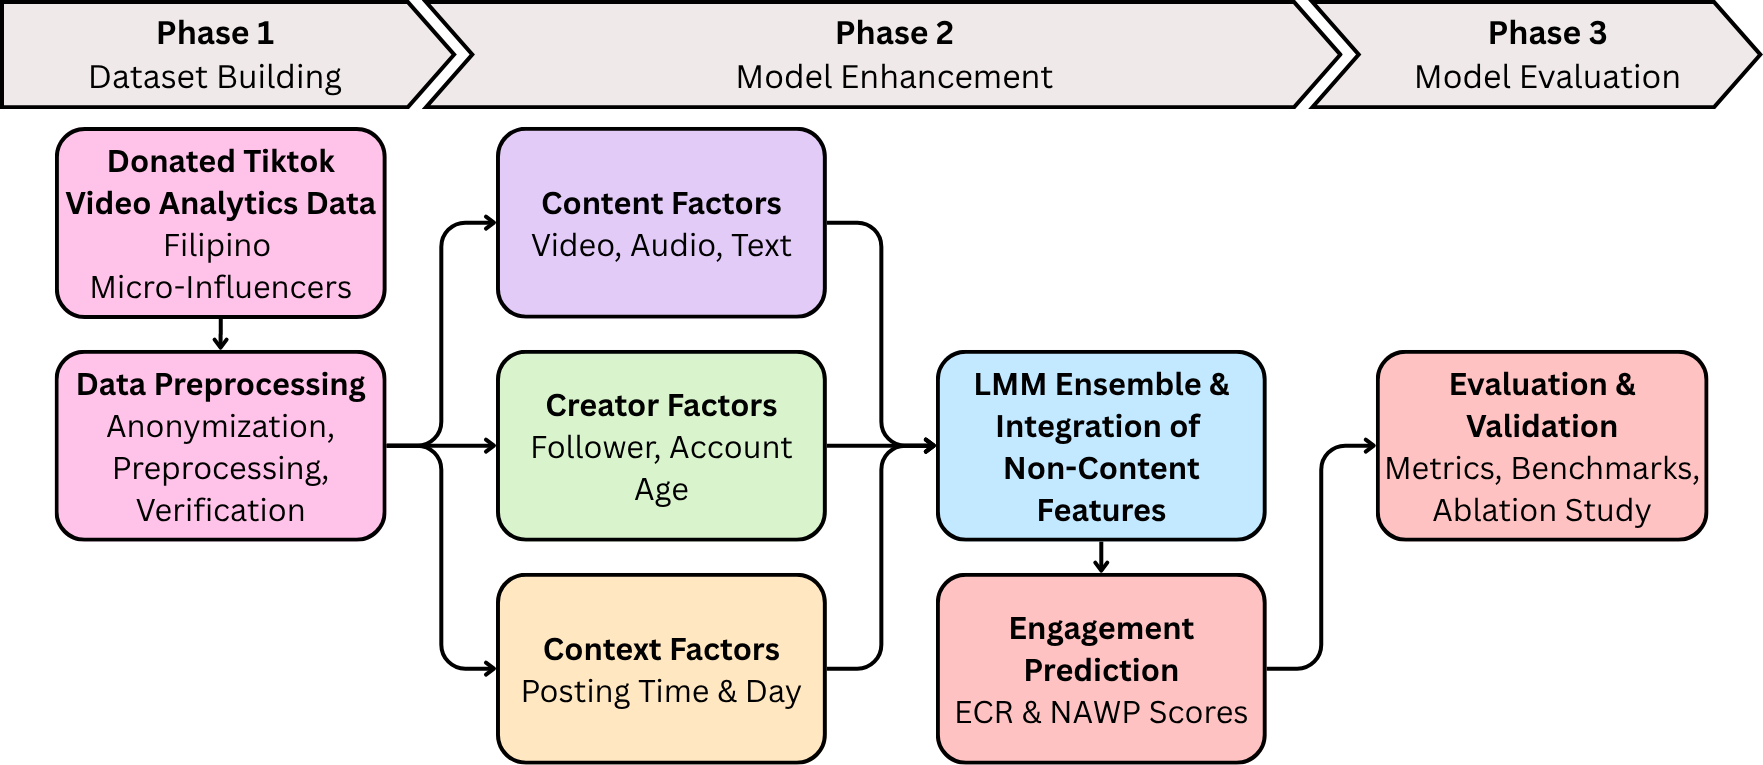
\includegraphics[width=1\linewidth]{figures/chap4/methodology_overview.png}
    \caption[Methodology Overview]
    {The high-level end-to-end pipeline. Donated data goes through preprocessing, then the three feature layers (content, creator, context) combine on the LMM ensemble before producing the \hl{ECR and NAWP scores} that gets validated and evaluated.}
    \label{fig:methodology_overview}
\end{figure}

The proposed methodology as shown in Figure \ref{fig:methodology_overview} follows a multi-phase pipeline designed to investigate the influence of content, creator, and contextual features on short-form video engagement. In Phase 1, we build the dataset, MicroTok-PH. It begins with donated TikTok analytics data sourced from Filipino micro-influencers, which then undergoes preprocessing, including anonymization, formatting, and verification steps to ensure the cleanliness and reputability of the dataset. The data is then separated into three feature categories that go in the core of Phase 2: development of our model C3-LMM. Content factors, which capture the video's visuals, audio, and text modalities; Creator factors, which account for creator-level signals such as follower count and account age; and Context factors, which include situational variables such as the posting time and day. These three feature categories converge into a Large Multimodal Model (LMM) Ensemble that integrates the non-content features alongside the content-based representations, allowing C3-LMM to reason jointly across the three feature categories. A prediction is then made based on the integrated representation that outputs \hl{an Engagement Continuation Rate (ECR) score, and a Normalized Average Watch Percentage derived from the ECR. These two scores} serve as the quantitative targets C3-LMM will be trained to predict. Finally, Phase 3 entails the C3-LMM Evaluation stage of the pipeline, where the C3-LMM's performance is assessed through standard evaluation metrics, benchmarks, and an ablation study.

%While the current pipeline utilizes a specific Large Multimodal Model (LMM) architecture and a defined set of initial features, this approach is intended to be iterative and flexible. The research acknowledges that data representations and model configurations may be refined as the donated TikTok archives are processed. Consequently, while the procedures detailed in this section represent the primary technical path, the study maintains the scope to explore alternative modeling techniques or additional feature signals to ensure the most robust analysis of the engagement data.

\section{Building the MicroTok-PH Dataset}

The construction of the MicroTok-PH will address two gaps in existing short-form video (SFV) benchmarks. Content-only datasets such as SnapUGC lack the creator-specific and contextual metadata required for cold-start prediction \cite{li2024delving}. Automated scraping, the alternative most often used to enlarge a benchmark, produces inconsistent labels and cannot reach the backend retention metrics that platforms expose only to verified account holders \cite{li2025vquala}. This study will work around both limits through a data donation approach in which Filipino micro-influencers voluntarily submit their first-party analytics. The donation route gives the study verified ground-truth labels and avoids any access pattern that would conflict with platform terms.

\subsection{Data Acquisition and Collection}

\subsubsection{Participants and Video Criteria}
\label{sec:participants}

The target participants of this study are active Filipino TikTok content creators who maintain a professional account and at least 18 years old. Following the justification established in Section~2.5, recruitment is restricted to the micro-influencer tier, and 30 to 50 creators will be recruited by email through purposive sampling against the eligibility criteria defined below. Consenting creators must agree to share their videos and analytics from the past year for the purposes of this research. The professional account requirement is a technical prerequisite rather than a stylistic one, as the platform-verified backend metrics on which this study depends (ECR and NAWP) are exposed only to such accounts through TikTok Studio.

\paragraph{Inclusion Criteria.} A creator is eligible only if all of the following conditions are met:
\begin{itemize}
    \item Maintains between 10{,}000 and 100{,}000 TikTok followers at the time of screening.
    
    \item Is at least 18 years of age.

    \item Demonstrates an active and consistent posting history over the preceding six months, operationalized as a minimum of three published videos per week.

    \item Produces content primarily in English, Tagalog, or Taglish.

    \item Operates an account with TikTok Analytics enabled and exportable, permitting first-party export of per-video ECR and NAWP metrics via TikTok Studio.
\end{itemize}

\paragraph{Exclusion Criteria.} An account is excluded at the creator level, and individual videos are excluded at the content level, under the following conditions:
\begin{itemize}
    \item \textit{Account level:} The account holds fewer than 10{,}000 followers, placing it in the nano-influencer tier, or more than 100{,}000 followers, placing it in the macro-influencer tier or above---whether at screening or if the threshold is crossed during the collection window.

    \item \textit{Content level:} A video employs Text-to-Speech (TTS) narration, is a compilation, is AI-generated, or is an unoriginal re-upload.
\end{itemize}

\paragraph{Video Content Criteria.} For a creator's donation to be admissible, the submitted archive must satisfy all of the following:
\begin{itemize}
    \item Comprise a historical archive of 20 to 30 videos (a minimum of 20 per
    creator), each accompanied by platform-verified analytics.

    \item Contain only videos that have been live for at least one month.

    \item Contain only videos uploaded within the past year.
\end{itemize}

Collectively, these criteria constrain the sample to authentic, original, and analytically stable creator content while admitting the full range of naturally occurring formats so that the model is trained on a representative slice of the short-form ecosystem. This isolates the content-, creator-, and context-level variation that C3-LMM is designed to model from the algorithmic amplification, synthetic media, and metric instability that would otherwise confound pre-publication engagement prediction.

\subsubsection{Material}

Two materials will be used for data acquisition and collection: a Chrome extension for downloading analytics data, and a website for data submission.

\noindent\textbf{Chrome Extension: TikTok Analytics Exporter}

The creators will be provided with a Chrome extension entitled TikTok Analytics Exporter upon recruitment that allows them to export their video analytics history as a Comma-Separated Value (CSV) file. A detailed explanation about the extension can be found in Chapter \ref{sec:TikTok Analytics Exporter}.

Shown in Figure \ref{fig:analytics_exporter} is the TikTok Analytics Exporter interface. Its features include extracting analytics on a per-video basis and the follower count history of the creator.

\begin{figure}[h]
    \centering
    
\includegraphics[width=0.5\linewidth]{chap4/tiktok-analytics-exporter.png}
    \caption[TikTok Analytics Exporter Interface]
    {The TikTok Analytics Exporter popup, showing the two export controls a creator uses to download their per-video analytics and follower-count history as CSV files.}
    \label{fig:analytics_exporter}
\end{figure}

Two CSV files can be generated through the exporter: (a) per-video analytics that includes video\_id, post\_date, post\_time, caption, ECR, NAWP, etc.; and (b) follower count history that contains the total follower count and net count on a per-day basis for the last year. The fields and descriptions of the respective generated CSV files can be found in Tables \ref{tab:video_performance_csv} and \ref{tab:follower_history_csv}.

Every export performed with the TikTok Analytics Exporter is carried out by the creator, on the creator's own account, and is limited to data they are already entitled to access under TikTok's Privacy Policy \mbox{\cite{tiktok_privacy_2026}}. The extension reads the analytics that TikTok Studio already exposes to the logged-in creator and writes them to a CSV on the participant's local disk \cite{tiktok_tos_2026}. It runs entirely inside the creator's own authenticated browser session: the extension does not bypass any access control, does not store credentials, does not contact any remote endpoint, and does not collect viewer-level data. Each participant exercises the access right granted to users under TikTok's Privacy Policy ``Your Rights and Choices'' clause \cite{tiktok_privacy_2026}. The extension only automates the export the creator is already entitled to perform manually.

Scraping, as the term is used in the SFV benchmark literature, describes the automated harvesting of data belonging to other users, typically by traversing public pages at scale and without the participation of the account holder \cite{li2025vquala}. The exporter operates under the opposite conditions. It runs inside the creator's own browser, on the creator's own authenticated session, and only while the creator is on their own TikTok Studio pages; it never enumerates other accounts and never traverses public content. Each export begins with a deliberate action by the creator, who presses the export control in the extension popup and receives the resulting CSV file as a download on their own machine. No party other than the creator gains access to the account, and no data leaves that machine until the creator chooses to upload the files through TokDrop. The research team is therefore not a third party reaching into a creator's account, but the recipient of files the creator produced and sent. What the exporter automates is a retrieval the creator is entitled to perform by hand, resting on the creator's right to access their own information under the Privacy Policy ``Your Rights and Choices'' clause \cite{tiktok_privacy_2026} and exercised on first-party data alone.

Two backup strategies are prepared in case the exporter cannot run on a participant's device.

\begin{itemize}
    \item \textbf{Saved-page export.} The creator opens their TikTok Studio analytics page and saves it through the browser's own \mbox{``Save page as''} function, then uploads the resulting HTML file through TokDrop. The research team parses the saved file offline to recover the fields listed in Tables \mbox{\ref{tab:video_performance_csv}} and \mbox{\ref{tab:follower_history_csv}}. Nothing runs against TikTok in this path; the creator produces a static copy of a page they are already viewing.

    \item \textbf{Manual entry.} The creator reads the per-video figures from TikTok Studio and enters them into a spreadsheet template supplied by the research team, together with a screenshot of each analytics panel for verification. This path is the slowest and yields fewer videos per participant, but it removes automation from the collection entirely.
\end{itemize}

Both paths lower the number of videos a single participant can realistically contribute, so each is applied per participant rather than as a general substitute for the exporter.

\noindent\textbf{Collection Website: TokDrop}

Creators who agree to donate their video and analytics data may do so through our collection website, TokDrop. Figure \ref{fig:tokdrop_ui} presents screenshots of the steps the creator takes while using the website.

TokDrop will be distributed to creators via email, along with their access code for authorization. Here, creators first have to input their provided access code before they can read the Informed Consent Form (found in Appendix A), agree to provide their data for this study, and upload the CSV files downloaded from the TikTok Analytics Exporter.

  \begin{figure}[htbp]
      \centering

      \begin{subfigure}{\textwidth}
          \centering
          
\includegraphics[width=\textwidth, height=0.42\textheight, keepaspectratio]{chap4/TokDrop-1.png}
          \caption{Step 1 --- Access code: the creator unlocks the form with the code from their invitation email.}
          \label{fig:tokdrop_ui_a}
      \end{subfigure}

      \bigskip

      \begin{subfigure}{\textwidth}
          \centering
          
\includegraphics[width=\textwidth, height=0.42\textheight, keepaspectratio]{chap4/TokDrop-2.png}
          \caption{Step 2 --- Informed consent: the full consent form is shown and must be agreed to before continuing.}
          \label{fig:tokdrop_ui_b}
      \end{subfigure}

      \caption[TokDrop User Interface]{The four-step submission flow of the TokDrop collection website: access-code entry, informed consent, CSV
  upload, and confirmation.}
      \label{fig:tokdrop_ui}
  \end{figure}

  \begin{figure}[htbp]\ContinuedFloat
      \centering

      \begin{subfigure}{\textwidth}
          \centering
          
\includegraphics[width=\textwidth, height=0.42\textheight, keepaspectratio]{chap4/TokDrop-3.png}
          \caption{Step 3 --- CSV upload: the creator uploads the two exporter files, the video-analytics CSV and the follower-history CSV.}
          \label{fig:tokdrop_ui_c}
      \end{subfigure}

      \bigskip

      \begin{subfigure}{\textwidth}
          \centering
          
\includegraphics[width=\textwidth, height=0.42\textheight, keepaspectratio]{chap4/TokDrop-4.png}
          \caption{Step 4 --- Confirmation: a confirmation screen acknowledges the submission was received.}
          \label{fig:tokdrop_ui_d}
      \end{subfigure}

      \caption[TokDrop User Interface]{The four-step submission flow of the TokDrop collection website: access-code entry, informed consent, CSV
  upload, and confirmation. \emph{(continued)}}
  \end{figure}

The data submitted will be stored on a private institute server and will be retained for two years after the completion of this study.

\subsubsection{Protocol}
\label{sec:protocol}

This section outlines the protocol for the entire data collection process, from participant recruitment to withdrawal. An overview of the timeline can be found in Figure \ref{fig:protocol}.

\begin{figure}[h]
    \centering
    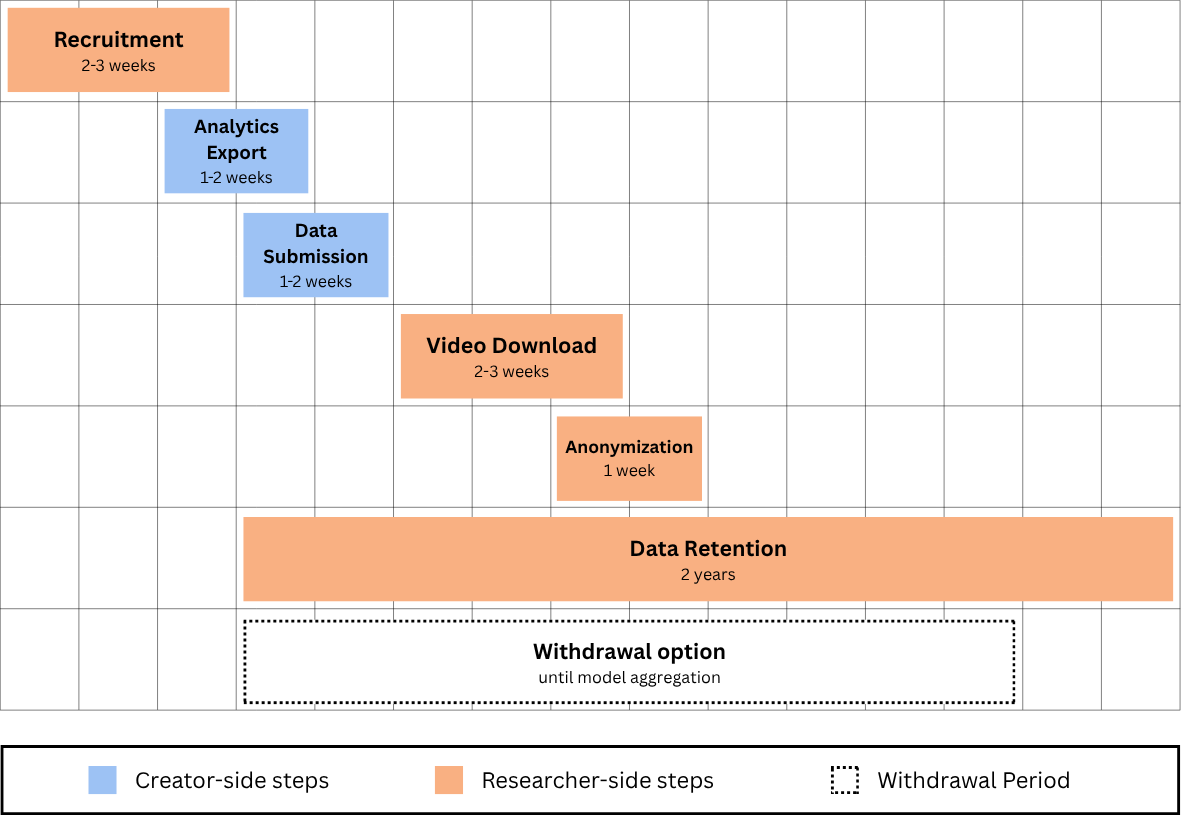
\includegraphics[width=1\linewidth]{figures/chap4/protocol.png}
    \caption[Data Collection Protocol Timeline]
    {Timeline of the data collection protocol, tracing the sequence from participant recruitment and consent through data donation, anonymization, and withdrawal handling.}
    \label{fig:protocol}
\end{figure}

\textbf{Participant Recruitment.} We create a list of candidate creators based on the criteria listed in Section \ref{sec:participants}. Candidates enter this list through two channels: direct outreach, in which we contact creators who appear to meet the criteria without prior introduction, and snowball sampling, in which creators who have completed their donation refer peers from their own network. Once selected, creators are approached through an email that introduces the study and explains its objectives, eligibility criteria, and the activities required of participants. The email outlines the voluntary nature of participation, provides a summary of the privacy and confidentiality measures of the study, and includes the contact information of the researchers for inquiries. It also contains the necessary participation resources, including the informed consent form, the TikTok Analytics Exporter extension, the link to TokDrop, and the unique access code required to upload the requested data. Referred creators are screened against the same criteria in Section \ref{sec:participants} and receive the same email and participation resources as those contacted directly, so participation remains voluntary through both channels. A copy of the email template can be found in Appendix C.

\textbf{Analytics Export.} The participant installs the TikTok Analytics Exporter Chrome extension (refer to Section \ref{sec:ext_installation}) and authenticates through their own TikTok account. Then, the creator will navigate to the appropriate page so that the extension can extract the relevant analytics (which is explained in Sections \ref{sec:ext_video_export} and \ref{sec:ext_follower_export}). Once extracted, the data can be downloaded as CSV files on the creator's local disk as a personal backup of their analytics.

% \textbf{Informed Consent.} The creator reviews the research objectives, the data handling policy, and the likeness clause covering donated footage before providing a digital signature. The consent form is attached as Appendix A and is signed before any donation step proceeds.

\textbf{Data Submission.} If the creator agrees to donate their data for the research, they can log in to TokDrop, using the access code provided by the researchers. The creator first reads the informed consent form (found in Appendix A) where they can review the research objectives, data privacy, the likeness clause regarding their videos, and participation requirements. The informed consent form covers the use of the creator's likeness as part of the retrieved videos. C3-LMM performs engagement prediction and does not perform face recognition or other biometric inference. Secondary subjects appearing incidentally in the background of retrieved footage are covered by the same clause, since the creator confirms standing to authorize the retrieval of their videos at the time of consent. As a part of the participation requirements, creators must enable public visibility and TikTok's download permission on their posted videos before proceeding to the submission step. These settings must remain active through the completion of the video downloading step done by the researchers. After agreeing, they can upload the downloaded CSV files obtained from the extension.

\textbf{Video Download.} The research team downloads each video through TikTok's built-in download option on the creator's public video page, locating each post using the video IDs contained in the submitted CSV files. The filename for each downloaded video will be ``$\langle \texttt{video\_id}\rangle$\texttt{.mp4}''. This step is performed only for creators who have provided informed consent and satisfied the participation requirements. Video retrieval operates on publicly accessible content that the creator has explicitly made downloadable, in compliance with TikTok's Terms of Service \cite{tiktok_tos_2026}. The study does not scrape, access non-public data, or bypass platform access controls at any stage.

\textbf{Anonymization.} Researchers strip identifying fields from the analytics CSV (account handle, profile name, contact email) and replace the creator handle with a randomized alphanumeric ID. The mapping between the original handle and the anonymized ID is held separately from the working MicroTok-PH dataset, under the ethical safeguards stated the informed consent form.

\textbf{Data Retention.} Non-anonymized donor information is held for a maximum of two years from the first publication of any result derived from the dataset or from project completion, whichever is later. Anonymized data is held for a maximum of three years on the same basis. After each retention window, the corresponding files are deleted, and the anonymization mapping table is deleted at the close of the two-year window so that no path remains from anonymized rows back to the original creator.

\textbf{Withdrawal.} A participant may withdraw their donation at any time before the final model aggregation by contacting the proponent email listed in the consent form. After identity is verified through the original donation record, the participant's data is deleted. %across the ingestion portal, the working dataset, and the long-term archive.

\textbf{Legal and Terms-of-Service Basis.} The entire data collection process rests on the creator's right to access their own information. Under TikTok's Privacy Policy \mbox{``Your Rights and Choices''} clause \mbox{\cite{tiktok_privacy_2026}}, each participating creator is entitled to access and obtain a copy of the analytics TikTok holds about their own content. Every step above, namely analytics export, data submission, and video download, operates only on first-party data the creator is already entitled to view and on public videos the creator has explicitly made downloadable. The study does not scrape other users' data, access non-public information, or bypass any platform access control \mbox{\cite{tiktok_tos_2026}}. For the same reason, recruitment is limited to professional accounts and excludes TikTok Business accounts. Section 8(a)(ii)(1) of TikTok's Business Terms of Service prohibits Business account holders from sharing \mbox{``TikTok Data''} with any third party, where that term covers data, analytics, or reports on the performance of the Platform \mbox{\cite{tiktok_business_tos_2026}}. Excluding Business accounts keeps that restriction outside the scope of the donation without reducing the data available, since the required per-video metrics are exposed to professional accounts through TikTok Studio.

\subsection{Dataset Preparation}

The resulting MicroTok-PH dataset will integrate three primary feature categories, which serve as the initial framework for representing short-form video engagement. The Multimodal Content category will consist of raw MP4 video files, captions, and hashtags. The Creator-Related category will incorporate metadata including follower counts and account age. The Contextual category will be represented by specific posting timestamps. This study will use our model, C3-LMM, to automatically extract and separate the visual and acoustic signals from raw MP4 files. 

Acknowledging the potential for evolving data representations, this feature set remains flexible and subject to refinement based on the specific attributes available within the donated TikTok archives. While these represent the primary variables for the study, the methodology allows for the inclusion of additional signals. A comprehensive list of these initial features is provided in Table \ref{tab:feature_list}.

\begin{table}[H]
    \centering
    \begin{tabular}{ll}
        \toprule
        \textbf{Feature}  & \textbf{Category} \\
        \midrule
        Raw MP4 File  & Multimodal Content \\
        Follower Count  & Creator-Related \\
        Creator Age  & Creator-Related \\
        Posting Time  & Contextual \\
        Posting Day  & Contextual \\
        \bottomrule
    \end{tabular}
    \caption{High-Level List of Initial Input Features}
    \label{tab:feature_list}
\end{table}

Each analytics row will be verified against its corresponding downloaded video. The \texttt{video\_id} from the CSV is matched to the downloaded MP4 filename to confirm a one-to-one correspondence. Rows that lack a corresponding MP4 will be flagged for manual review and are excluded from the final MicroTok-PH dataset.

Following the verification process, the dataset will be reviewed for duplicate entries, incomplete analytics, corrupted files, and inconsistent metadata before being formatted into the final MicroTok-PH schema. Potentially anomalous records will be manually examined to distinguish legitimate viral content from data quality issues. Only records determined to contain inconsistencies or errors will be excluded, while valid high-performing or viral videos will be retained to preserve the natural engagement distribution of the dataset.

Raw video files and their associated analytics metadata will be formatted to the schema described in Table \ref{tab:schema}. Once the finalized MicroTok-PH dataset has been constructed, it will be partitioned into mutually exclusive training, validation, and testing subsets using a creator-disjoint stratified split. Specifically, 70\% of the creators will be assigned to the training set, 15\% to the validation set, and the remaining 15\% to the testing set. Under this strategy, all videos contributed by a single creator are assigned exclusively to one partition, preventing information leakage arising from creator-specific characteristics such as editing style, audience demographics, and posting behavior. The creator-level split will be stratified according to follower-count tiers (e.g., lower-, middle-, and upper-range micro-influencers) so that each partition contains approximately the same proportion of creators from each tier. This preserves the follower-count distribution across the training, validation, and testing subsets, ensuring that each partition remains representative of the target micro-influencer population (10,000--100,000 followers). The 70/15/15 partition provides sufficient data for model training while reserving independent subsets for hyperparameter tuning and unbiased performance evaluation, making it a widely adopted practice in supervised machine learning. The resulting dataset structure is summarized in Table \ref{tab:schema}:

\begin{table}[H]
    \centering
    \begin{tabular}{llp{8cm}}
        \toprule
        \textbf{Field}  & \textbf{Data Type} & \textbf{Description} \\
        \midrule
        video\_id  & String & Unique video id \\
        creator\_id  & String & Unique, anonymized creator id \\
        caption & String & Caption associated with the video \\
        follower\_count & Number & Creator's follower count on posting date \\
        day\_sin & Number & Sine-encoded position of the posting day in the weekly cycle \\
        day\_cos & Number & Cosine-encoded position of the posting day in the weekly cycle \\
        time\_sin & Number & Sine-encoded position of the posting time in the daily cycle \\
        time\_cos & Number & Cosine-encoded position of the posting time in the daily cycle \\
        % post\_day & String & Day of the week when the video was posted \\
        % post\_time & Time & Time when the video was posted \\
        days\_since\_first\_post & Number & Number of days between the creator's first post and the current video's posting date. \\
        \bottomrule
    \end{tabular}
    \caption{MicroTok-PH Data Schema for Raw Videos and Associated Analytics Metadata}
    \label{tab:schema}
\end{table}

follower\_count and days\_since\_first\_post will be normalized to a mean of $\mu=0$ and a standard deviation of $\sigma=1$. The day and time of posting will be represented through cyclical encoding to preserve their periodic nature. 


% \subsection{Data Cleaning and Quality Assurance}

% \hl{Before feature extraction, the collected data will undergo a data cleaning process to ensure consistency and reliability. Records with missing or corrupted video files, incomplete analytics, duplicate entries, or inconsistent metadata will be excluded from the dataset. In addition, summary statistics and visual inspection techniques, such as box plots and z-score analysis, will be used to identify potential outliers arising from exceptional viral events or anomalous engagement behavior. Flagged samples will be manually reviewed to distinguish legitimate viral content from erroneous or inconsistent records. Only samples determined to be invalid or unrepresentative will be removed, and all exclusions will be documented to ensure transparency and reproducibility.}

% NOT INCLUDED - this is a part of the model already
 % For each input video, exactly eight keyframes are uniformly sampled across the video duration to focus on the initial ``hook'' window. Each frame is resized to a resolution of $384 \times 384$ for VideoLLaMA2 and $768 \times 28 \times 28$ for Qwen2.5-VL. Background audio will be converted into spectrograms to capture emotional and narrative cues.

% \subsection{Ethical Safeguards and Limitations}

% Ethical integrity is maintained through the procedures stated in the informed consent form (Appendix A) and the Ethics Review Form.

% \textbf{Public availability and downloads.} The informed consent form (Appendix A) includes a requirement that participants enable public visibility and TikTok's download permission on their posted videos before proceeding to the submission step. These settings must remain active through the completion of the video retrieval step.

% \textbf{Identity and likeness.} Creator handles are replaced with randomized identifiers at the anonymization step, and the original-to-anonymized mapping is held separately from the working dataset. The informed consent form covers the use of the creator's likeness as part of the retrieved frames; the proposed model performs engagement prediction and does not perform face recognition or other biometric inference. Secondary subjects appearing incidentally in the background of retrieved footage are covered by the same clause, since the creator confirms standing to authorize retrieval of the footage at the time of consent.

% \textbf{Data retention.} Non-anonymized donor information is held for a maximum of two years from the first publication of any result derived from the dataset or from project completion, whichever is later. Anonymized data is held for a maximum of three years on the same basis. After each retention window, the corresponding files are deleted, and the anonymization mapping table is deleted at the close of the two-year window so that no path remains from anonymized rows back to the original creator.

% \textbf{Withdrawal.} A participant may withdraw their donation at any time before the final model aggregation by contacting the proponent email listed in the consent form. After identity is verified through the original donation record, the participant's data is deleted across the ingestion portal, the working dataset, and the long-term archive.

% \textbf{TikTok platform compliance.} The analytics export step is initiated by the creator, performed inside the creator's own authenticated browser session, and limited to data the creator is already entitled to access \cite{tiktok_privacy_2026, tiktok_tos_2026}. The extension does not bypass any access control, does not store credentials, and does not contact any remote endpoint. Video retrieval in Step 4 operates on publicly accessible content that the creator has explicitly made downloadable, in compliance with TikTok's Terms of Service \cite{tiktok_tos_2026}. The study does not scrape, access non-public data, or bypass platform access controls at any stage.


\section{Developing C3-LMM}

The engagement prediction framework proposed in this study extends beyond content-only analysis by integrating multimodal context features with creator and contextual metadata. This section describes C3-LMM, the Large Multimodal (LMM) ensemble that serves as our evaluator for multimodal content, and the approaches for incorporating creator and contextual features.

\subsection{LMM Ensemble Architecture}

The core of C3-LMM is an ensemble of two frozen LMM backbones, both of which act as a feature extractor that processes raw SFV content and produces engagement predictions per video. VideoLLaMA2 was selected for spatiotemporal and auditory understanding, and Qwen2.5-VL for visual-semantic reasoning. These two models were selected for their complementary capabilities. This architecture follows the approach of \citeauthor{sun2025engagement} \citeyear{sun2025engagement}, who demonstrated that this ensemble of independently trained LLMs yields more accurate engagement predictions than a single model.

Both models are used with the frozen pre-trained weights from \citeauthor{sun2025engagement} \citeyear{sun2025engagement}. The weights are frozen due to computational constraints and because they were already trained on SFVs, which is the domain of the study. Fine-tuning the LMM backbones using the MicroTok-PH dataset can be done in the future.


% The framework will leverage an ensemble of state-of-the-art LMMs to capture diverse engagement signals:
% \begin{itemize}
%     \item \textbf{VideoLLaMA2 Branch:} An audio-visual-language model will be utilized for joint spatiotemporal and auditory understanding. It will process key video frames, background sound, and textual metadata simultaneously.
%     \item \textbf{Qwen2.5-VL Branch:} A vision-language model will focus on general visual-semantic reasoning. It will provide complementary reasoning using keyframes and text-based metadata.
% \end{itemize}

\subsubsection{Ensemble Strategy}

The two LMM backbones act as independent prediction models. Each model processes the same input video and produces an engagement score for each target metric: Engagement Continuation Rate (ECR) and Normalized Average Watch Percentage (NAWP). The final ensemble prediction for a given video is computed as the mean of the two models' predictions:
\begin{equation}
    \hat{y}_{ensemble} = \frac12(\hat{y}_{VideoLLaMA2} + \hat{y}_{Qwen2.5-VL})
\end{equation}
where $\hat{y}_{VideoLLaMA2}$ and $\hat{y}_{Qwen2.5-VL}$ represent the predicted scores of the respective model for a given target metric. This simple averaging strategy follows the approach of \cite{sun2025engagement}. Weighted ensemble methods, wherein the contribution of each model is scaled by a learned coefficient, can be explored in future work.

\subsection{Integration of Creator and Contextual Features}
\label{sec:feature_integration}

The primary enhancement of this study will be the inclusion of non-content variables to address the informational deficit in traditional cold-start modeling. While standard LMMs reason primarily about the media file, C3-LMM will augment those embeddings with structured metadata available at the time of upload:
\begin{itemize}
    \item \textbf{Creator Influence:} Follower count and account age will be integrated to account for the social influence and creator-audience relationships that bias initial distribution.
    \item \textbf{Contextual Timing:} Posting day and time will be incorporated to model the impact of peak user activity on early engagement probabilities.
\end{itemize}

This study proposes two approaches to integrating these non-content features.

\subsubsection{Approach 1: Prompt-Based Feature Injection}
\label{sec:approach_1}

In this prompt-based approach, each frozen LMM backbone is zero-shot prompted. Creator and contextual features are formatted as natural language and injected directly into the text prompt provided to each LMM alongside the video input, with no fine-tuning or parameter updates done to any model. An overview of this approach is shown in Figure \ref{fig:approach_1_overview}.

\begin{figure}[h]
    \centering
    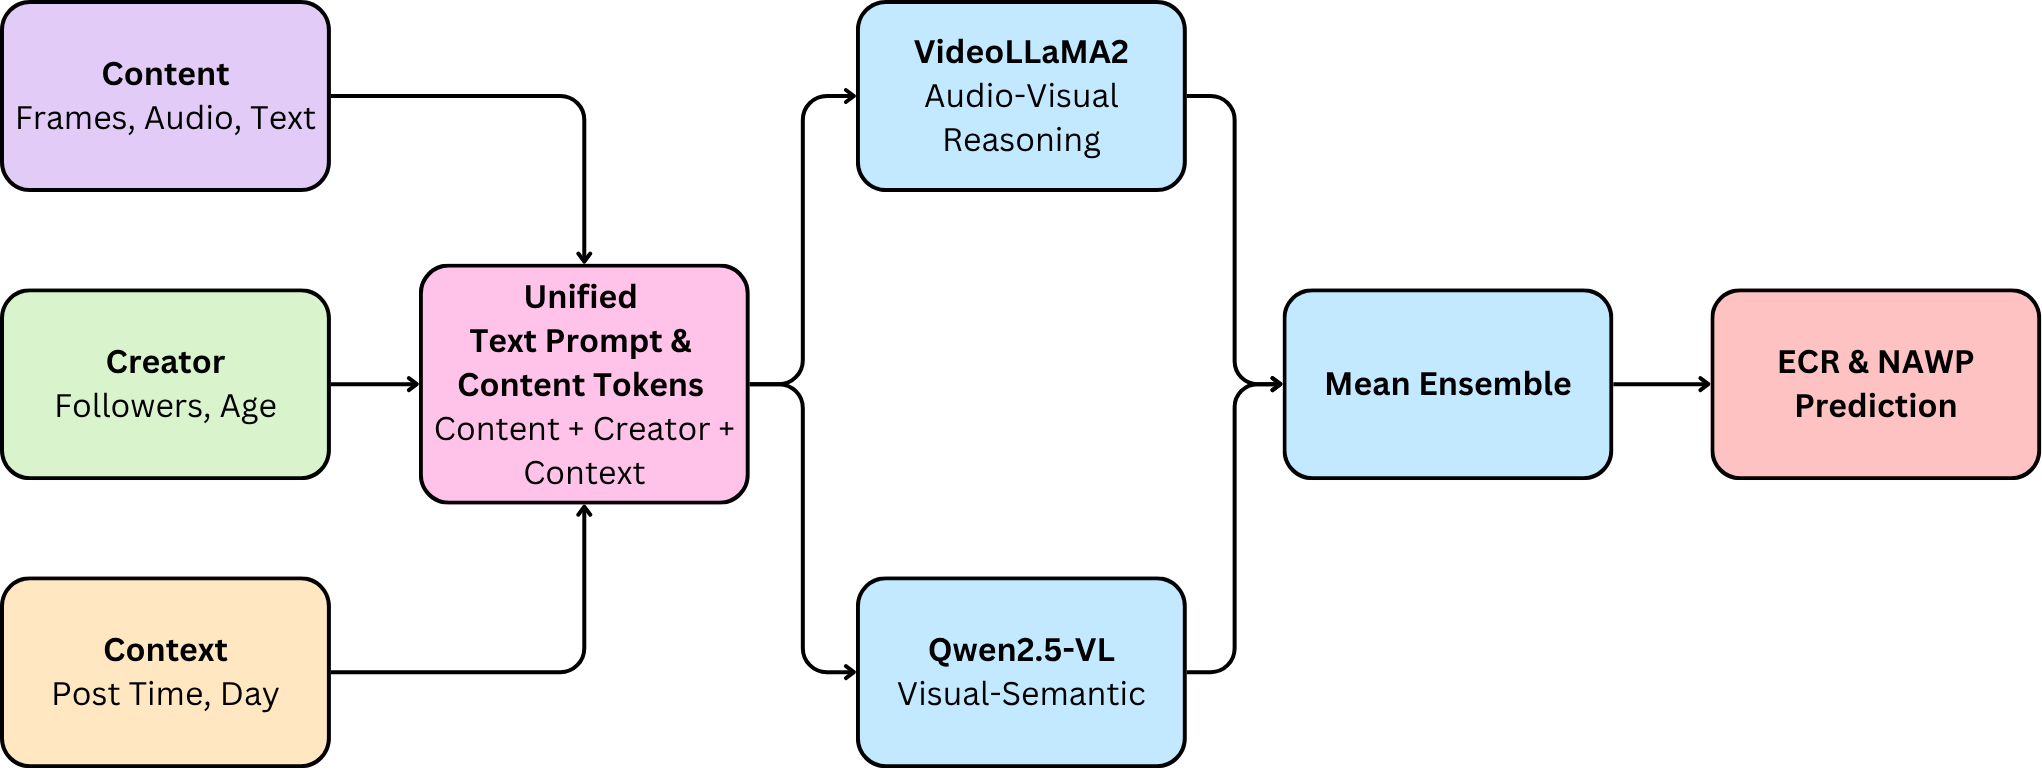
\includegraphics[width=1\linewidth]{figures/chap4/approach_1.png}
    \caption[Overview of the Prompt-Based Feature Injection Approach]
    {Overview of the prompt-based approach: structured creator and context features are converted to text and fused into the LMM prompt with the video, producing the prediction in a single pass.}
    \label{fig:approach_1_overview}
\end{figure}

One conversation will be made with the models for each input video. The model's expected output will be its predicted values for ECR and NAWP. The only prompt it will be given is:

\begin{quote}
\small
``How would you judge the engagement continuation rate and the normalized average watch percentage of the following content, where engagement continuation rate represents the probability of watch time exceeding 5 seconds. 

\smallskip
\noindent The video frames: $\langle\texttt{frames\_tokens}\rangle\langle\texttt{frames\_tokens}\rangle\dots\dots\langle\texttt{frames\_tokens}\rangle$. \\
The audio: $\langle\texttt{audio\_tokens}\rangle$. \\
The caption: $\langle\texttt{caption}\rangle$. \\
The follower count: $\langle\texttt{follower\_count}\rangle$. \\
The post date: $\langle\texttt{post\_date}\rangle$. \\
The post time: $\langle\texttt{post\_time}\rangle$. \\
The number of days between the creator's first post and the current video's posting date: $\langle\texttt{days\_since\_first\_post}\rangle$.''
\end{quote}

If the data is not available or not included, it will be replaced with a \texttt{None} value. Additionally, since we are making one conversation per video, the context window limit of the LMM models will not be reached.

This approach leverages the language understanding capabilities of the frozen LMM backbones to perform cross-modal reasoning across all available feature types in a single forward pass, without any fine-tuning done on the models. Because the models are zero-shot prompted, all creator and contextual features are expressed in natural language so that the pre-trained weights can directly interpret them. This presents the LMM with a unified prompt that contextualizes the video context with creator- and contextual-level information, allowing the model to weigh content and context jointly when generating its prediction.

\subsubsection{Approach 2: Auxiliary Model Ensemble}
\label{sec:approach_2}

In the auxiliary model approach shown in Figure \ref{fig:approach_2_overview}, a separate Multilayer Perceptron (MLP) will be trained exclusively on the creator and contextual features of our training set. The MLP operates independently of the LMM backbones, producing its own engagement prediction. The final prediction is then computed by ensembling the auxiliary model's output with the LMM ensemble prediction, through a weighted average:
\begin{equation}
    \hat{y}_{\text{final}} = \alpha \cdot \hat{y}_{\text{LMM\_ensemble}} + (1 - \alpha) \cdot \hat{y}_{\text{auxiliary}}
\end{equation}
where $\alpha \in [0, 1]$ controls the relative contribution of the multimodal content analysis and the additional feature analysis.

\begin{figure}[h]
    \centering
    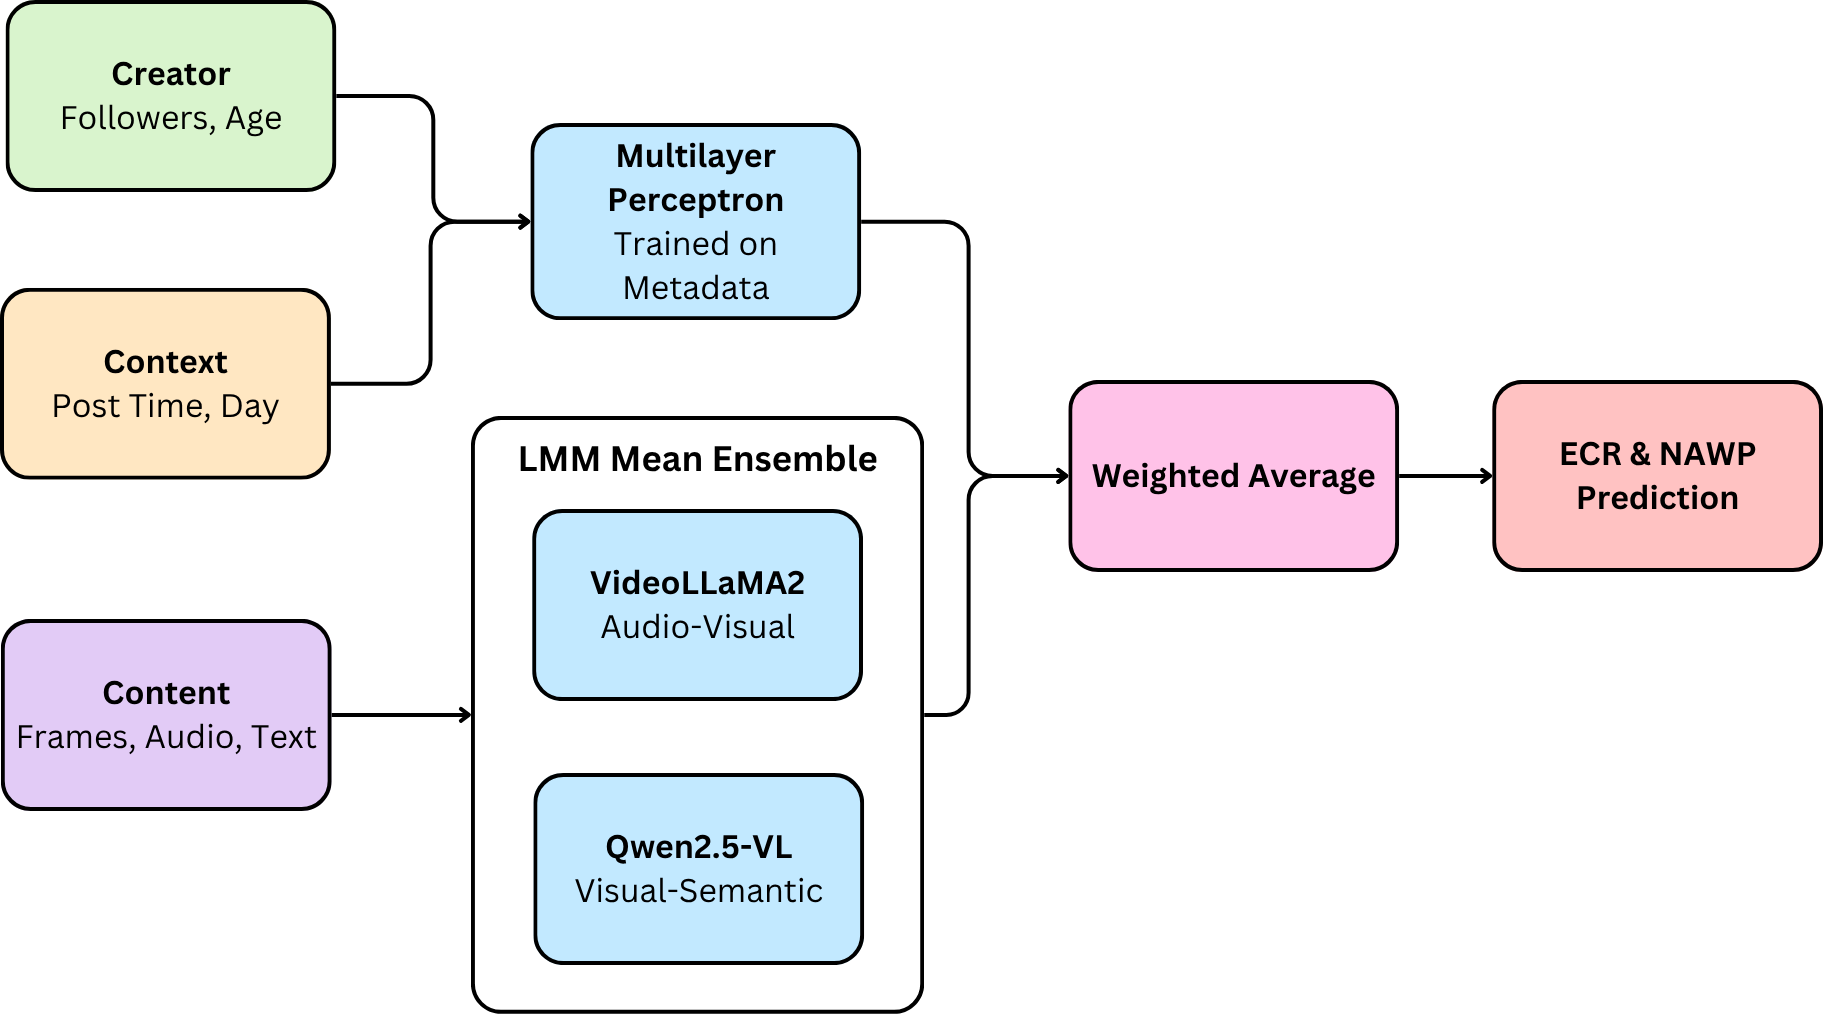
\includegraphics[width=1\linewidth]{figures/chap4/approach_2.png}
    \caption[Overview of the Auxiliary Model Approach for integrating creator and contextual features]
    {Overview of the auxiliary approach: a content stream (LMM) and a metadata stream (MLP) are computed independently and merged through a weighted late fusion controlled by $\alpha$.}
    \label{fig:approach_2_overview}
\end{figure}

The hyperparameters of the MLP, including the number of hidden layers, number of neurons per layer, learning rate, batch size, activation function, optimizer, and number of training epochs, will be tuned during the development of C3-LMM to identify the configuration that yields the best validation performance based on our validation set.

This approach has the advantage of decoupling content understanding from contextual processing, allowing each component to be trained and evaluated independently. It also provides interpretability benefits, as the auxiliary model's feature importances can be inspected to understand which creator-level factors most influence engagement predictions. However, it introduces additional engineering complexity and does not benefit from cross-modal reasoning between content and context features.

\section{Evaluating C3-LMM}

To evaluate the performance of C3-LMM, it will be compared to current benchmark models. It will be evaluated using the same metrics as those models.

\subsection{Evaluation Metrics}

C3-LMM's objective is to predict the ECR and NAWP of a given short video. ECR is the probability that the user will watch a video after 5 seconds. NAWP measures the retention of the user, regardless of video length.

This study will assess C3-LMM using the Root Mean Squared Error (RMSE) of both ECR and NAWP, the Spearman Rank Correlation Coefficient (SRCC), and the Pearson Linear Correlation Coefficient (PLCC). A final score is computed using both SRCC and PLCC: 
\begin{equation}
    \text{Final Score} = 0.6\times SRCC + 0.4\times PLCC
\end{equation}

\subsection{Comparison of Feature Integration Approaches}

Before comparing C3-LMM against external benchmarks, the two feature integration strategies introduced in Section \ref{sec:feature_integration} must first be compared against each other. Approach 1 (Prompt-Based Feature Injection) incorporates creator and contextual metadata directly into the language prompt alongside content embeddings, allowing the LMM to perform cross-modal reasoning. Approach 2 (Auxiliary Model Ensemble) instead keeps content and metadata processing separate, training a dedicated MLP on structured creator and contextual features and fusing its output with the LMM output. The goal of this comparison is to identify which approach yields better prediction performance, so that only the winning approach is used in the subsequent benchmark comparison and ablation study.

Both approaches will be evaluated on the same test set, and compared using a Wilcoxon signed-rank test to see if there is a statistically significant difference in the prediction accuracy of each approach. 

\subsubsection{Evaluation Procedure}

The same held-out test set will be used to evaluate each approach to ensure a fair comparison. Both approaches will produce predictions for the same set of $N$ test videos, resulting in paired predictions that can be used for direct comparison on a per-video basis.

For each test video $i$, both approaches produce predicted values $\hat{y}_i^{(\text{ECR})}$ and $\hat{y}_i^{(\text{NAWP})}$ for each target metric. The per-video absolute prediction error for each approach is computed as:
\begin{equation}
    e_i^{(a)} = |y_i - \hat{y}_i^{(a)}|, \quad a \in \{\text{ECR}, \text{NAWP}\}
\end{equation}
where $y_i$ is the ground-truth value for video $i$. This produces two paired error vectors, $\mathbf{e}^{(\text{ECR})}$ and $\mathbf{e}^{(\text{NAWP})}$, each of length $N$, for each target metric.

% \hl{To minimize evaluation bias and ensure that the reported performance reflects true model generalization, the dataset will be partitioned into 70\% training, 15\% validation, and 15\% testing using a creator-disjoint split. Under this partitioning strategy, all videos contributed by a single creator are assigned exclusively to one partition. Consequently, no creator will appear in more than one subset. This prevents information leakage arising from creator-specific characteristics, such as visual style, editing patterns, audience demographics, or posting behavior, which could otherwise artificially inflate predictive performance. By evaluating the model only on creators that were not encountered during training, the reported results more accurately represent the model's ability to generalize to unseen creators in real-world deployment.}

In addition to the per-video errors, the aggregate metrics defined in the previous section are computed for each approach: the RMSE of ECR and NAWP, the SRCC and PLCC between predicted and ground-truth values, and the Final Score.

\subsubsection{Statistical Testing}

A Wilcoxon signed-rank test will be used to determine whether there is a statistically significant difference in the paired per-video absolute errors between the two approaches. For each target metric (ECR and NAWP), the null hypothesis $H_0$ is that the median of the paired differences $d_i = e_i^{(\text{ECR})} - e_i^{(\text{NAWP})}$ is zero. The alternative hypothesis $H_1$ is that the median paired difference is not zero. The test is conducted at a significance level of $\alpha = 0.05$.

\subsubsection{Decision Criteria}

The selection of the winning approach is depicted in Figure \ref{fig:decision_tree}. The selection is based on both the aggregate evaluation metrics and the statistical test results. If the Wilcoxon signed-rank test yields a statistically significant result ($p < 0.05$) for at least one target metric, the approach with the lower median per-video error for that metric is selected. If both metrics yield significant results favoring the same approach, the decision is straightforward. In the event of conflicting results across ECR and NAWP, the approach with the higher Final Score is preferred, as this composite measure balances ranking accuracy and prediction precision. If the test does not reveal a statistically significant difference for either metric, the approach with the higher Final Score is selected as the default.

\begin{figure}[h]
    \centering
    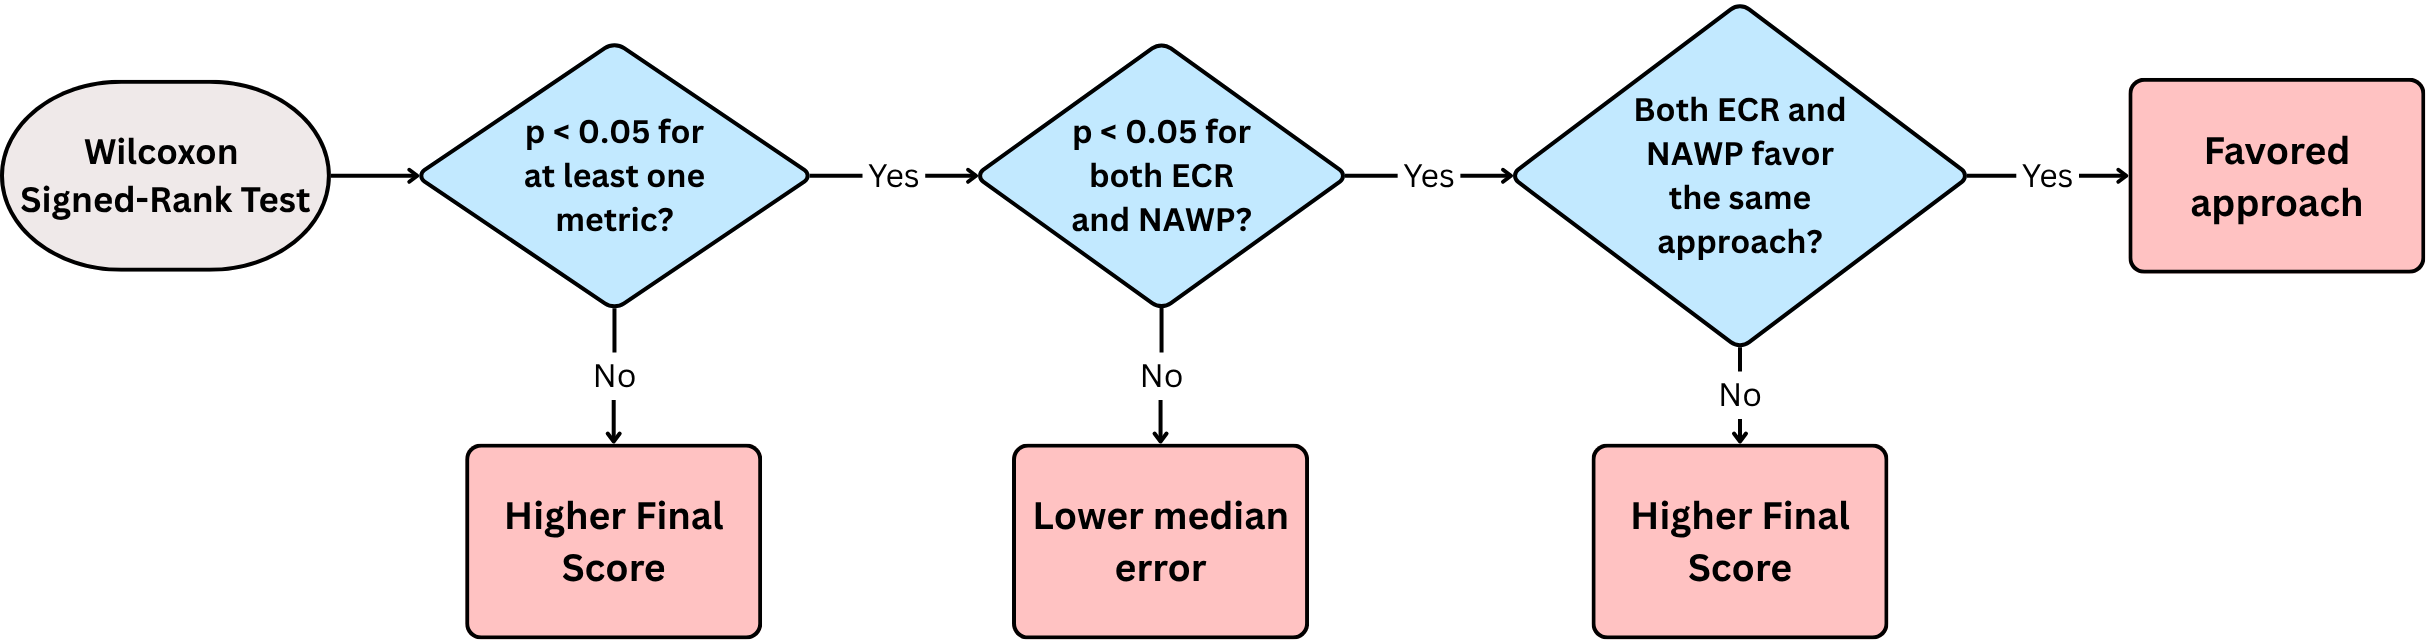
\includegraphics[width=1\linewidth]{figures/chap4/decision_tree_approach.png}
    \caption[Decision Tree for Choosing the Better Approach]
    {Decision flowchart for selecting between the prompt-based and auxiliary approaches, branching on the Wilcoxon signed-rank outcomes for ECR and NAWP and, when they conflict, the Final Score.}
    \label{fig:decision_tree}
\end{figure}

Once the winning approach is identified, subsequent evaluations, specifically the benchmark comparison and the ablation study, will be conducted exclusively on that approach. Evaluating both approaches through the full downstream pipeline would double the computational cost of inference and statistical testing without providing additional insight, since the purpose of this initial comparison is precisely to eliminate the redundancy of carrying forward a demonstrably inferior or statistically indistinguishable alternative.

\subsection{Benchmark Comparison}

Our study will use the models LMM-EVQA by \citeauthor{sun2025engagement} and MMF-QE by \citeauthor{guan2025mmf} as our benchmarks for comparison. We chose these because they are the best performing models available in predicting user engagement for SFVs in cold-start scenarios \cite{li2025vquala}.

As shown in Figure \ref{fig:sun2025_framework}, LMM-EVQA by \citeauthor{sun2025engagement} utilized an ensemble of two LMMs: VideoLLaMA2 \cite{cheng2024videollama}, which is an LMM designed for audio-visual and spatio-temporal understanding, and Qwen2.5-VL \cite{wang2024qwen2}, which is a vision-language model.

\begin{figure}[h]
    \centering
    
\includegraphics[width=1\linewidth]{chap4/sun2025_framework.png}
    \caption[LMM-EVQA (Sun et al., 2025) Framework Overview]
    {Ensemble framework of LMM-EVQA for predicting SFV engagement, combining VideoLLaMA2 for audio-visual and spatio-temporal understanding with Qwen2.5-VL for vision-language reasoning \cite{sun2025engagement}.}
    \label{fig:sun2025_framework}
\end{figure}

On the other hand, MMF-QE by \citeauthor{guan2025mmf} predicted ECR with the use of a collaborative framework of three branches as shown in Figure \ref{fig:guan2025_framework}: (1) a foundational model extracting multimodal features, (2) a disentangled model for technical and aesthetic factors based on DOVER \cite{wu2023exploring}, and (3) an instruction-tuned Qwen2.5-VL model.

\begin{figure}[h]
    \centering
    
\includegraphics[width=1\linewidth]{chap4/guan2025_framework.png}
    \caption[MMF-QE (Guan et al., 2025) Framework Overview]
    {MMF-QE is a three-branch collaborative framework for engagement prediction, integrating multimodal feature extraction, DOVER-based technical and aesthetic disentanglement, and instruction-tuned Qwen2.5-VL \cite{guan2025mmf}.}
    \label{fig:guan2025_framework}
\end{figure}

The goal of this comparison is to determine whether the integration of creator and contextual features in C3-LMM produces prediction errors that are statistically significant from those of the content only benchmark models, LMM-EVQA and MMF-QE. Two separate hypotheses are formulated, one for each benchmark. They will be tested independently of each other.

\subsubsection{Evaluation Procedure}

All three models (C3-LMM, LMM-EVQA, and MMF-QE) will be evaluated on the same held-out test set of $N$ videos to ensure a fair comparison. Each model will produce predictions for every test video, resulting in paired predictions that allow direct per-video comparison between C3-LMM and each benchmark.

For each test video $i$ and each model $m \in \{\text{C3-LMM}, \text{LMM-EVQA}, \text{MMF-QE}\}$, the per-video absolute prediction error is computed as:
\begin{equation}
    e_i^{(m)} = |y_i - \hat{y}_i^{(m)}|
\end{equation}
where $y_i$ is the ground-truth value for video $i$ and $\hat{y}_i^{(m)}$ is the predicted value from model $m$. This error is computed separately for each target metric (ECR and NAWP), producing paired error vectors of length $N$ for each model pair.
In addition to the per-video errors, the aggregate metrics will be computed for each model: the RMSE of ECR and NAWP, the SRCC and PLCC between predicted and ground-truth values, and the Final Score.

\subsubsection{Statistical Testing}

Two separate hypotheses are formulated, one for each benchmark model:
\begin{itemize}
    \item \textbf{Hypothesis 1 (C3-LMM vs.\ LMM-EVQA):} The null hypothesis $H_0^{(1)}$ states that the median of the paired differences $d_i = e_i^{(\text{C3-LMM})} - e_i^{(\text{LMM-EVQA})}$ is zero. The alternative hypothesis $H_1^{(1)}$ states that the median paired difference is not zero.
    \item \textbf{Hypothesis 2 (C3-LMM vs.\ MMF-QE):} The null hypothesis $H_0^{(2)}$ states that the median of the paired differences $d_i = e_i^{(\text{C3-LMM})} - e_i^{(\text{MMF-QE})}$ is zero. The alternative hypothesis $H_1^{(2)}$ states that the median paired difference is not zero.
\end{itemize}
Each hypothesis will be tested independently using a Wilcoxon signed-rank test, conducted separately for ECR and NAWP. Because each hypothesis addresses a distinct benchmark model and constitutes an independent research question, no multiple-comparison correction is applied. Each test will be evaluated at a significance level of $\alpha = 0.05$.

\subsubsection{Interpretation of Results}

For each benchmark comparison, the results are interpreted following Figure \ref{fig:decision_tree_benchmark}.

If the Wilcoxon signed-rank test yields a statistically significant result ($p < 0.05$) for a given target metric, the model with the lower median per-video error for that metric is considered to have superior prediction accuracy. If both metrics yield significant results favoring the same model, that model is clearly the better performer for the comparison in question. In the event of conflicting results across ECR and NAWP, the model with the higher Final Score is considered superior, as this composite measure balances ranking consistency and prediction precision. If the test does not reveal a statistically significant difference for either metric, the models are considered comparable in performance, and the aggregate metrics are reported descriptively without claiming a definitive advantage.

\begin{figure}[h]
    \centering
    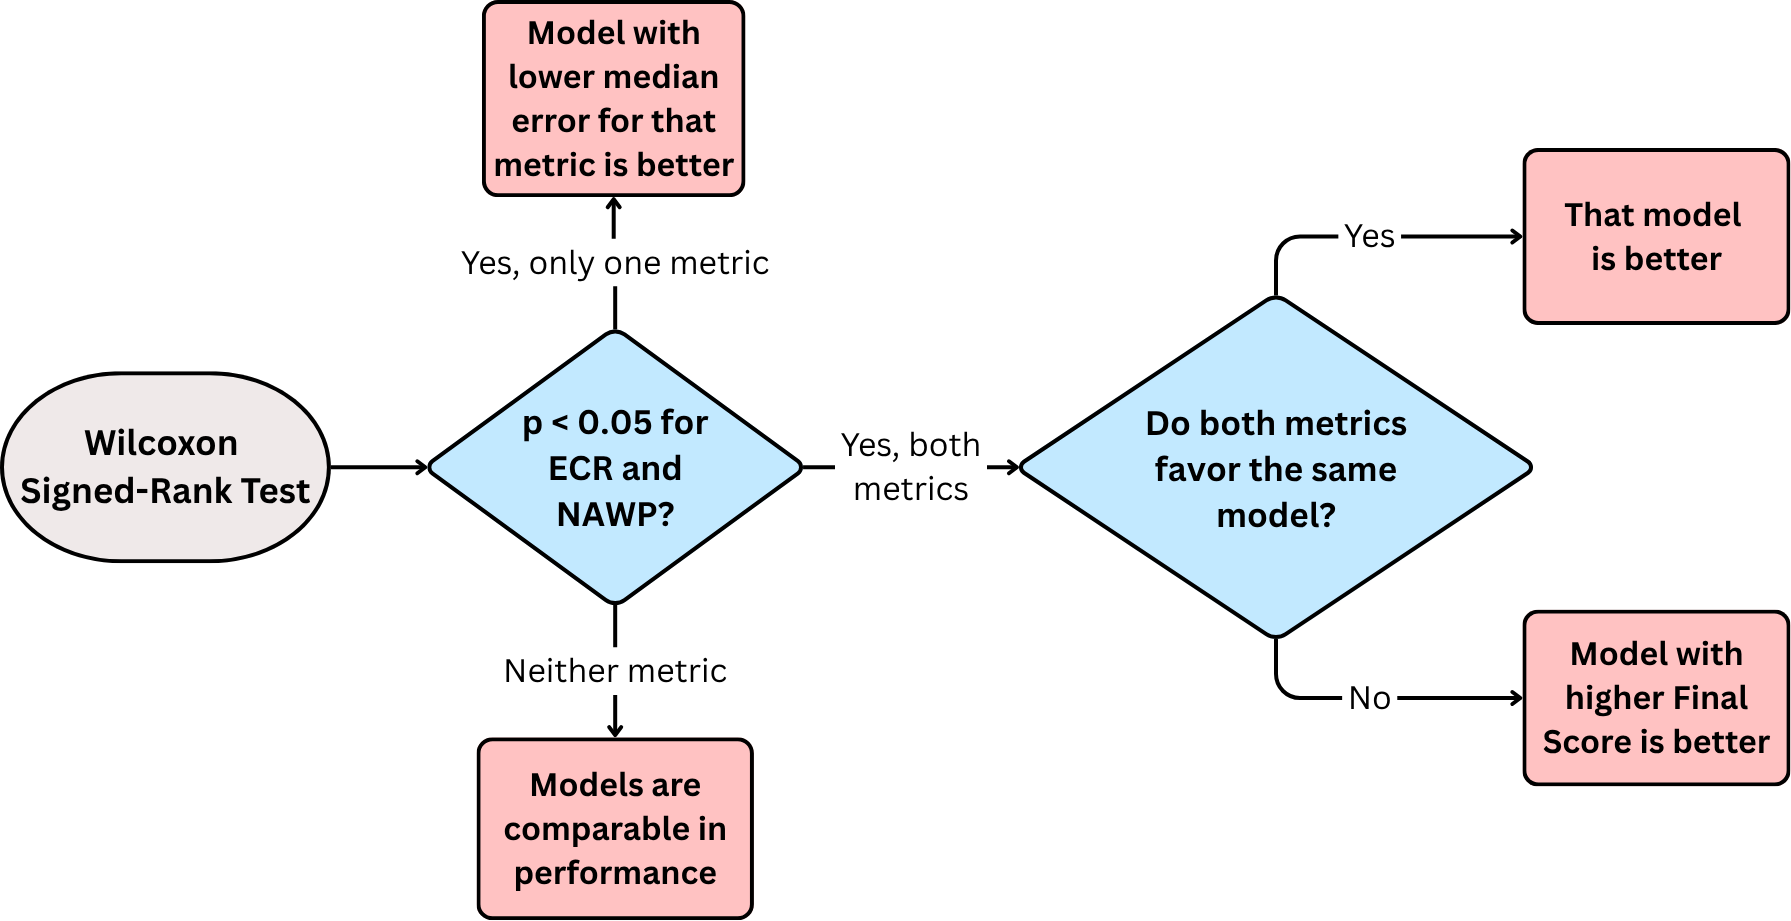
\includegraphics[width=1\linewidth]{figures/chap4/decision_tree_benchmark.png}
    \caption[Flowchart for interpreting the benchmark comparison tests]
    {Flowchart for interpreting the benchmark comparison, mapping each combination of ECR and NAWP Wilcoxon outcomes to a conclusion about whether C3-LMM outperforms the content-only benchmark.}
    \label{fig:decision_tree_benchmark}
\end{figure}

\subsection{Ablation Study}

To determine the impact of the proposed features on prediction accuracy, an ablation study will be conducted on the approach that yielded better results. These experiments will isolate or combine the different categories from Table \ref{tab:feature_list}: multimodal content $F_{content}$, creator features $F_{creator}$, and contextual $F_{context}$, into four model configurations, $M_0$ to $M_3$. $M_0$ (Baseline) uses content features only, $M_1$ (Creator-Augmented) adds creator features, $M_2$ (Context-Aware) adds contextual features, and $M_3$ (Fully Integrated) combines all three categories. In doing so, the impact of each factor on the prediction accuracy of the ECR and NAWP is quantitatively measured. Table \ref{tab:model_configurations} shows the configurations of each model.

\begin{table}[h]
    \centering
    \begin{tabular}{lccc}
        \toprule
        \textbf{Model} & $F_{content}$ & $F_{creator}$ & $F_{context}$ \\
        \midrule
         $M_0$: Baseline & \checkmark &  &  \\
         $M_1$: Creator-Augmented & \checkmark & \checkmark &  \\
         $M_2$: Context-Aware & \checkmark &  & \checkmark \\
         $M_3$: Fully Integrated & \checkmark & \checkmark & \checkmark \\
        \bottomrule
    \end{tabular}
    \caption[Model Configurations for Ablation Studies]
    {Four model configurations used in the ablation study, each combining a different subset of content, creator, and contextual features to isolate their individual and joint contribution to ECR and NAWP prediction accuracy}
    \label{tab:model_configurations}
\end{table}

This ablation study tests the hypothesis: \textit{The integration of creator features ($F_{creator}$) and contextual features ($F_{context}$) with multimodal content features ($F_{content}$) produces a statistically significant difference in the prediction errors of ECR and NAWP compared to using only content features.}

\subsubsection{Evaluation Procedure}

All four model configurations will be evaluated on the same held-out test set of $N$ videos to ensure a fair comparison. Each configuration will produce predictions for every test video, resulting in paired predictions that allow direct per-video comparison between each augmented model and the content-only baseline.

For each test video $i$ and each configuration $M_k$, $k \in \{0, 1, 2, 3\}$, the per-video absolute prediction error is computed as:
\begin{equation}
    e_i^{(M_k)} = |y_i - \hat{y}_i^{(M_k)}|
\end{equation}
where $y_i$ is the ground-truth value for video $i$ and $\hat{y}_i^{(M_k)}$ is the predicted value from configuration $M_k$. This error is computed separately for each target metric (ECR and NAWP), producing paired error vectors of length $N$ for each configuration pair.

In addition to the per-video errors, the aggregate metrics are computed for each configuration: the RMSE of ECR and NAWP, the SRCC and PLCC between predicted and ground-truth values, and the Final Score.

\subsubsection{Statistical Testing}
Three pairwise comparisons are conducted against the baseline model $M_0$, each testing whether the addition of a specific feature group produces a statistically significant difference in prediction errors:
\begin{itemize}
    \item \textbf{Comparison 1 ($M_0$ vs.\ $M_1$):} The null hypothesis $H_0^{(1)}$ states that the median of the paired differences $d_i = e_i^{(M_0)} - e_i^{(M_1)}$ is zero. The alternative hypothesis $H_1^{(1)}$ states that the median paired difference is not zero. This tests the effect of adding creator features.
    \item \textbf{Comparison 2 ($M_0$ vs.\ $M_2$):} The null hypothesis $H_0^{(2)}$ states that the median of the paired differences $d_i = e_i^{(M_0)} - e_i^{(M_2)}$ is zero. The alternative hypothesis $H_1^{(2)}$ states that the median paired difference is not zero. This tests the effect of adding contextual features.
    \item \textbf{Comparison 3 ($M_0$ vs.\ $M_3$):} The null hypothesis $H_0^{(3)}$ states that the median of the paired differences $d_i = e_i^{(M_0)} - e_i^{(M_3)}$ is zero. The alternative hypothesis $H_1^{(3)}$ states that the median paired difference is not zero. This tests the combined effect of all additional features.
\end{itemize}
Each comparison is conducted using a Wilcoxon signed-rank test, evaluated separately for ECR and NAWP. Since three pairwise comparisons are made against a common baseline, a Bonferroni correction is applied. The adjusted significance threshold is $\alpha = \frac{0.05}{3} \approx 0.0167$.

\subsubsection{Interpretation of Results}

For each pairwise comparison, the results are interpreted following Figure \ref{fig:decision_tree_ablation}.

If the Wilcoxon signed-rank test yields a statistically significant result ($p < 0.0167$) for a given target metric, the direction of the median error difference is inspected: a positive median difference ($e_i^{(M_0)} > e_i^{(M_k)}$) indicates that the augmented model reduces prediction error, while a negative difference indicates a degradation. If the test does not reveal a statistically significant difference ($p \geq 0.0167$), the added features are considered to provide no measurable benefit for that metric, and the aggregate metrics are reported descriptively.

\begin{figure}[h]
    \centering
    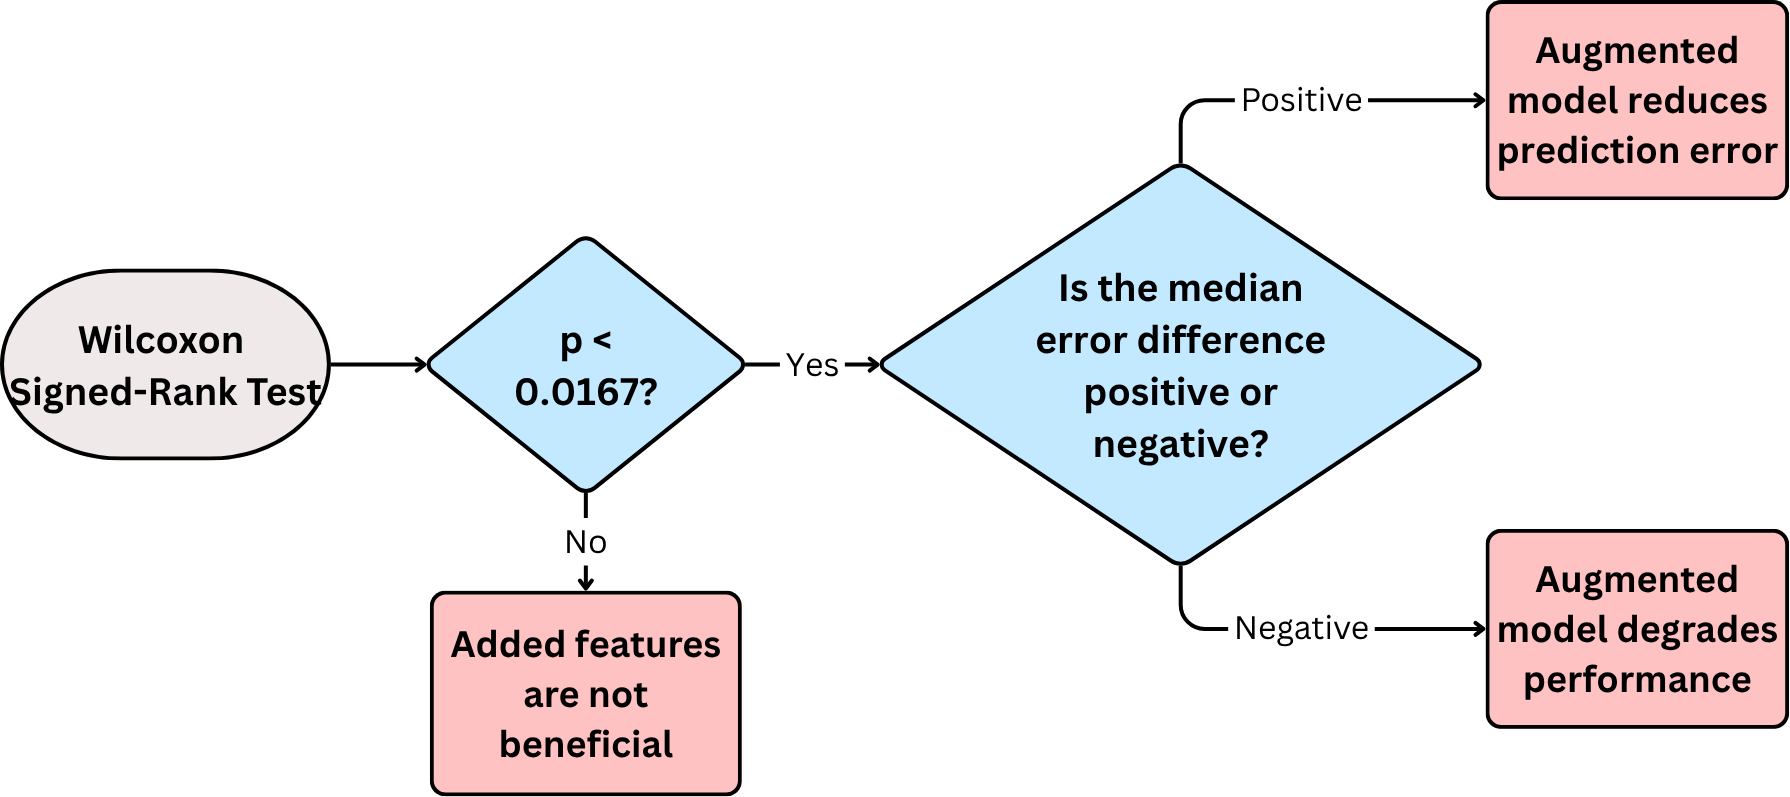
\includegraphics[width=1\linewidth]{figures/chap4/decision_tree_ablation.png}
    \caption[Flowchart for interpreting the ablation study tests]
    {Flowchart for interpreting each ablation comparison against baseline $M_0$, using the Bonferroni-corrected threshold ($\alpha$ = 0.0167) and the sign of the median error difference to classify a feature group as beneficial, harmful, or non-significant.}
    \label{fig:decision_tree_ablation}
\end{figure}

The matrix of outcomes across the three comparisons will reveal which feature category/categories contribute meaningful improvements to engagement prediction. If the fully integrated model $M_3$ yields a statistically significant improvement over $M_0$ while neither $M_1$ nor $M_2$ alone does, this would suggest a synergistic effect between creator and contextual features. Conversely, if one feature group consistently drives improvement while the other does not, this would indicate that the benefit is attributable to a specific category of metadata. These results will inform which feature groups are most impactful for predicting user engagement in cold-start scenarios.

\section{Calendar of Activities}

The proposed methodology will be done over the span of 12 months, divided into the three phases previously outlined.

The first phase will focus on gathering and preparing the data needed for the study. This includes selecting a group of creators, collecting their consent and data, and finally anonymizing, verifying, and cleaning the data. The Gantt Chart for this phase is found in Figure \ref{fig:gantt_phase_1}.

The second phase will focus on feature extraction, C3-LMM training, enhancement, and initial evaluation. Testing on the benchmark models will also occur here. The Gantt Chart for this phase is found in Figure \ref{fig:gantt_phase_2}.

The last phase will be the evaluation of the proposed model and conducting an ablation study. The Gantt Chart for this phase is found in Figure \ref{fig:gantt_phase_3}.

\begin{landscape}
\begin{figure}
    \centering
    
\includegraphics[width=1\linewidth]{chap4/gantt-phase-1.png}
    \caption{Gantt chart for Phase 1 (Dataset Building), creator selection, consent and data collection, and anonymization/verification/cleaning.}
    \label{fig:gantt_phase_1}
\end{figure}

\begin{figure}
    \centering
    
\includegraphics[width=1\linewidth]{chap4/gantt-phase-2.png}
    \caption{Gantt chart for Phase 2 (Model Development), feature extraction, C3-LMM training and enhancement, and initial benchmark testing.}
    \label{fig:gantt_phase_2}
\end{figure}

\begin{figure}
    \centering
    
\includegraphics[width=1\linewidth]{chap4/gantt-phase-3.png}
    \caption{Gantt chart for Phase 3 (Evaluation), final model evaluation and the ablation study.}
    \label{fig:gantt_phase_3}
\end{figure}
\end{landscape}

